
%
\documentclass[%
 reprint,
%superscriptaddress,
%groupedaddress,
%unsortedaddress,
%runinaddress,
%frontmatterverbose, 
%preprint,
%preprintnumbers,
%nofootinbib,
%nobibnotes,
%bibnotes,
 amsmath,amssymb,
 aps,
%pra,
%prb,
%rmp,
%prstab,
%prstper,
%floatfix,
]{revtex4-2}
\usepackage{natbib}
\usepackage{graphicx}% Include figure files
\usepackage{dcolumn}% Align table columns on decimal point
\usepackage{bm}% bold math
%\usepackage{hyperref}% add hypertext capabilities
%\usepackage[mathlines]{lineno}% Enable numbering of text and display math
%\linenumbers\relax % Commence numbering lines

%\usepackage[showframe,%Uncomment any one of the following lines to test 
%%scale=0.7, marginratio={1:1, 2:3}, ignoreall,% default settings
%%text={7in,10in},centering,
%%margin=1.5in,
%%total={6.5in,8.75in}, top=1.2in, left=0.9in, includefoot,
%%height=10in,a5paper,hmargin={3cm,0.8in},
%]{geometry}

\begin{document}

%\preprint{APS/123-QED}

\title{Serial and Parallel Computing of Particle Distribution \\ in Potential Wells with Thermal Reservoir }% \\


\author{Samuel Quitian Gallego$^{1}$, Ana Sofia Marulanda Duque$^{1}$}
\email{samuel.quitiang@udea.edu.co, sofia.marulanda2@udea.edu.co}
\affiliation{%
 $^1$Faculty of Natural and Exact Sciences, Physics Department, Universidad de Antioquia}

\date{\today}

\begin{abstract}
Our study focuses on the adaptation of a Monte Carlo-based simulation for obtaining the energy distribution of particles within an array of potential wells in contact with a thermal reservoir. It
investigates the efficiency of the simulation when executed using both single-processor serial and parallel processing via SSH cluster connection. By dividing the algorithm into parallelized tasks, we explore the benefits of parallel computing, focusing on computational time and resource utilization. By comparing the two approaches, we demonstrate significant reductions in computing time with this method particularly for larger systems and higher temperatures. The final results use simultaneous runs to display average energy behaviour according to temperature increase, the same as the system's heat capacity.
Ultimately, our research contributes to a deeper understanding of particle dynamics and highlights the importance of advanced computational methods in statistical physics.


\end{abstract}

\keywords{Metropolis, Statistical Physics}
\maketitle

%\tableofcontents

\section{\label{sec:level1}INTRODUCTION}
Statistical physics seeks to comprehend the emergent phenomena in systems with many interacting components. For instance, the study of thermal systems involves higher complexity since it needs to account for individual particle interaction. In such scenarios, the number of possible configurations increases rapidly, making it a challenging task to search for analytical solutions \cite{machta_complexity_2006}.

Scientific research requires managing extensive datasets, sharing data, and facilitating collaboration. Therefore, it is necessary to have a strong computational infrastructure that can store and process information efficiently while minimizing costs and processing times. As an example the Large Hadron Collider at CERN analyzes data streams generated at a rate of GB per second. Streamlined data transfer protocols are essential due to the multitude of users requiring access to data with unique permission levels \cite{jesshope_computational_1986}, \cite{dingle_causality_1970}, \cite{an_science_2019}.

The utilization of \textit{Secure Shell SSH} clusters has become increasingly popular in recent years, as it provides researchers with a powerful tool for remote job execution and real-time data exploration. With this architecture, individual users can be allocated a dedicated node or batch job within a master cluster, allowing for collaboration and enhanced contributions to scientific research. Furthermore, parallel computing enables multiple tasks to be performed simultaneously, significantly reducing processing time. It's important to note that parallel computing also includes communication time between processors and the integration of results from each of them, which can be a critical factor in achieving optimal performance.

In our previous project \cite{hotboxes}, we utilized a Metropolis-based algorithm to examine particle distribution in an array of infinite potential wells connected to a thermal reservoir. Each well holds a single particle, and once equilibrium is attained, the energy distribution among particles follows a \textit{Maxwell-Boltzmann} distribution. Building on this foundation, the current study aims to integrate parallel processing protocols and techniques to boost simulation efficiency, diminish resource demands, and expedite computation speed.
We present an adaptation of the project utilizing two different approaches: \textit{serial processing} and \textit{MPI parallel processing}. We aim to evaluate their respective strengths and weaknesses in terms of simulation efficiency, resource utilization, and scalability to  similar scenarios
\cite{shi_optical_2020} \cite{neophytou_nanostructured_2019} \cite{tsatsulnikov_modulation_1997}.



\section{BACKGROUND}

\subsection{Parallel Programming}

Traditionally, programming has been designed for serial computation. A problem is broken down into a sequential set of instructions, which are then executed one after the other on a single processor. However, as computing needs have grown, parallel computing has become increasingly essential. Parallel computing involves the coordinated use of multiple computers to solve the problem simultaneously, it is divided into distinct parts that can be addressed concurrently. Each part is then further divided into a sequence of instructions and executed simultaneously on different CPU's. This approach can significantly improve performance and reduce execution time for large-scale computations. Additionally, a common control or coordination mechanism is employed to manage the parallel execution, ensuring that all parts work together seamlessly \cite{dalcin_mpi_2005}.

The primary measure of a computer algorithm's efficacy is its computation time. In serial processing, this is the total time from start to finish. In parallel processing, additional factors like user input, inter-processor communication, data aggregation, and output processing also contribute, sometimes exceeding the serial processing time.

\subsection{Monte Carlo-Metropolis Particle in a Hot Box}

\textit{Monte Carlo} simulations are computational methods that employ randomness and probabilistic sampling to address problems where deterministic solutions are difficult to obtain. They are highly effective and broadly applicable, particularly in optimization, system simulation, and data interpretation. The \textit{Metropolis} algorithm is a prominent example, widely used in statistical physics. In this case, it functions by generating a series of energy values consistent with a \textit{Maxwell-Boltzmann} distribution to derive an expected value for an observable of interest.
At its core, it uses  \textit{Markov Chain Monte Carlo (MCMC)}, which explores a system's phase space and samples configurations based on their Boltzmann weights. It operates by generating a sequential list of configurations, proposing changes iteratively, and accepting or rejecting them according to a probabilistic criterion. This method ensures equilibrium is reached and samples configurations based on their equilibrium probabilities, adhering to a detailed balance condition. In here, the likelihood of being in a particular state $P_{s}$ is determined by the system's energy $E_{s}$ and temperature.
\begin{equation}
        P_s=\frac{1}{Z} e^{-\beta E_s}, 
\end{equation}

where $\beta=1 / k T$ and $Z$ is the partition function. \\

\subsection{The Metropolis algorithm}

The proposed system on this work consist on an array of infinite potential wells, each one with a fixed maximum number of energy levels $nmax$ that is held constant for all the simulations. The potential wells are in contact with a thermal reservoir that dictates the dynamics of the system. \par
Is considered a potential well width $l$ for all the wells and a number of particles $N$ in contact with a thermal bath at a given temperature $T$. As the system approaches stationary state, its behavior can be observed in terms of energy occupation, levels distribution and average energy values.
In this case, the initial state of the system can be expressed as: 
$n_0 = (4, 3, 2, ..., 4)$
\par
\begin{figure}[h]
    \centering
    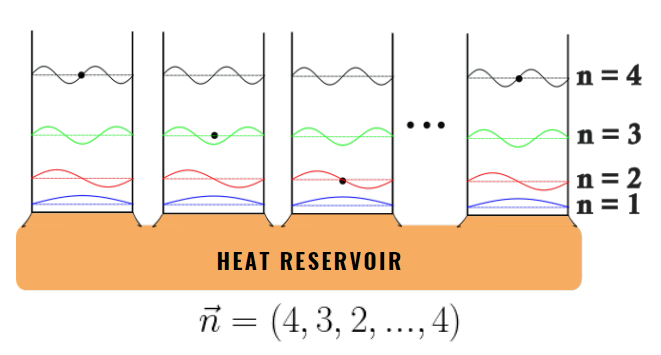
\includegraphics[width=0.4\textwidth]{reservoir.png} % Change 'example-image' to your image file name
    \caption{System of Infinite Potential Wells each one with one electron inside in a determine energy level, beneath the system scheme there is the initial vector state. }
    \label{fig:example}
\end{figure}

This algorithm employs acceptance ratios to determine the success of each iteration based on predefined criteria, iterating until the sampled states closely approximate the system's probability density. It relies on evaluating transition probabilities, representing changes from one state to another ($n_i \rightarrow n_j$). The likelihood of a particle descending to a lower energy level is influenced by its tendency to reach its ground state, while the probability of ascending to a higher energy level is influenced by $W$, which correlates with the thermal energy acquired from the reservoir. By accepting or rejecting proposed moves based on the acceptance ratio, the algorithm effectively traverses the state space, ultimately generating a statistically meaningful ensemble of configurations.

\begin{equation}
       W=P\left(n_i \rightarrow n_j\right)=\frac{p\left(E_{n_j}\right)}{p\left(E_{n_i}\right)}=\frac{e^{-\beta E_{n_j}} / Z}{e^{-\beta E_{n_i} / Z}}=e^{\beta\left(E_{n_j}-E_{n_i}\right)}.
\end{equation}

The method begins by generating a set of uniformly distributed random states. These states are subsequently evaluated against the probability distribution and transition criteria, undergoing the following test:
\begin{itemize}
    \item $r: random.uniform()<0.5$: probability of downward transition
    \item $r': random.uniform()<W$ if $r>0.5$: probability of upward transition
\end{itemize}

The simulation process involves calculating the energy difference between transitions and deciding to accept or reject them accordingly. The system is expected to reach a stationary state, where it maintains a consistent trend towards an average energy value, disregarding the initial random values generated.

After executing the code, it provides the average energy and the heat capacity. This facilitates further analysis by examining the relationship between the average energy, heat capacity, temperature, and well size. Such analysis helps understand the dependencies they have on the system's outcomes.

%--------------------------------------------------------------------------

\section{IMPLEMENTATION}
 \par
Two different implementations of the simulation code were developed in order to study the system's behavior. Initially, a \textit{Serial} approach was implemented, which provided an accurate first idea of how the system works. However, to improve computational efficiency, an additional implementation using \textit{MPI} was developed. 

\begin{itemize}
    \item {\textbf{Serial Computing:}} The initial version of the code operates sequentially, simulating the behavior of the system at each temperature one after the other. While straightforward to implement, this approach may lead to longer computation times, especially when exploring multiple iterations.
    \item {\textbf{SSH Cluster MPI4py:}} The most advanced implementation utilizes the \textit{Message Passing Interface (MPI)} through the mpi4py library to enable parallel processing on a distributed computing environment. Specifically, the code is designed to run on a cluster of computers connected via SSH protocol. MPI enables efficient communication and coordination among multiple computing nodes, allowing each node to simulate the behavior of the system for a specific initial conditions and temperatures, with the goal of having enough data to make a statistical analysis of the system. This parallelization strategy offers the highest level of performance scalability and is particularly well-suited for large-scale simulations involving extensive computational resources.
\end{itemize}

Each implementation provides unique benefits regarding computational efficiency and scalability, enabling thorough examination of the system's behavior across various temperatures. Ultimately, achieving consistency in results between both approaches is crucial for our objective of comprehending the impact of temperature on particle distribution and system stability.


\section{RESULTS and discussion}

\subsection{Serial Computing}

First, we run the simulation in a serial processing approach. From it, we see that the system exhibits high levels of stochastic and chaotic behaviour, resulting in various related outcomes with each run. The linear tendency on Fig \ref{fig:m4} is noticeable across cycles. However, as presented on Figure  \ref{fig:serialm4}, the heat capacity is the most varying quantity.

\begin{figure}[!h]
    \centering
    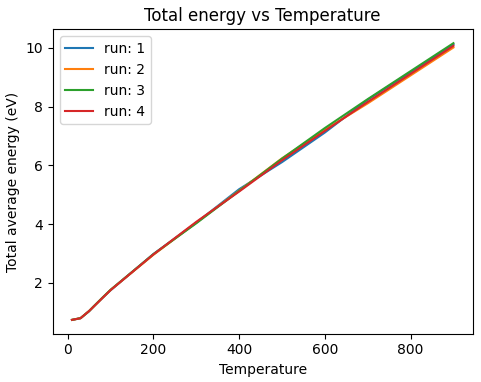
\includegraphics[width = 0.7\linewidth]{m4E.png}
    \caption{ Total average energy of the system at equilibrium respect to the temperature of the thermal bath for four different runs of the simulation.}
    \label{fig:m4}
\end{figure}

\begin{figure}[!h]
    \centering
    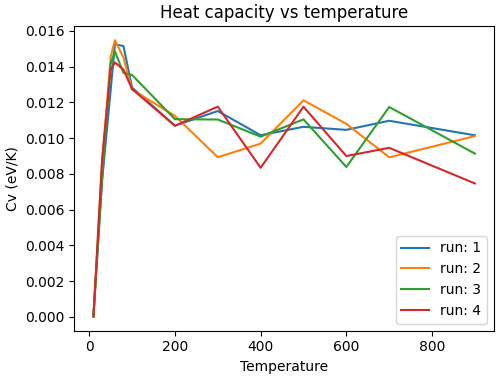
\includegraphics[width = 0.7\linewidth]{m4.png}
    \caption{Heat capacity of the system at equilibrium respect to the temperature of the thermal bath for four different runs of the simulation.}
    \label{fig:serialm4}
\end{figure}

To tackle this problem, we must conduct a statistical analysis of the system running the simulation multiple times and averaging the outcomes. This approach mitigates outliers, enhances analysis robustness, and improves the reliability of results across a wider range of data. In the context of serial computing, the processing time increases linearly with the increase in the amount of data to be processed.

\begin{figure}[!h]
    \centering
    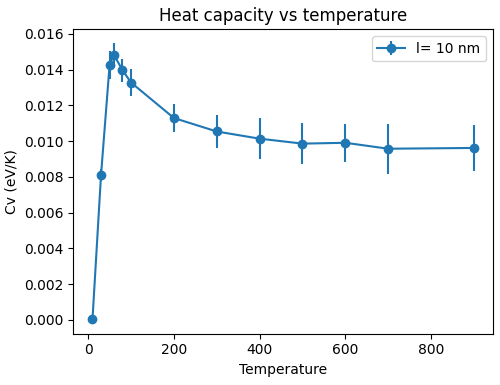
\includegraphics[width = 0.7 \linewidth]{Cvser.png}
    \caption{Curve of the average heat capacity of the system at equilibrium respect to the temperature of the thermal bath with its error bars, this curve is the result of the average heat capacity of 32 different runs of the simulation in a serial implementation.}
    \label{fig:cvser}
\end{figure}

As an example of this, we run the simulation of 200 potential wells 32 times with a \textit{For Cycle}, yielding an overall computing time of 1772.2 s. By averaging the results across cycles, the heat capacity graph depicted in Fig. \ref{fig:cvser} emerges, with error bars derived from the standard deviation ($\sigma$) of the data. As the dataset expands, the curve progressively smoothens across temperature values, accompanied by an increase in error bars. 





\subsection{MPI4py Paralell Computing}
When it comes to parallel computing, optimizing the performance of the computing unit is crucial. One way to achieve this is by removing graphical processes, which can consume a lot of RAM memory. By doing so, the simulation's output may differ from previous code, as the results of desired quantities are now stored as a dataframe in comma-separated values (.csv) in the local folder. If graphical processes and libraries are desired to be implemented, they should be used in a separate script that does not use MPI and imports the .csv results from the local folder.

\begin{figure}[h!]
    \centering
    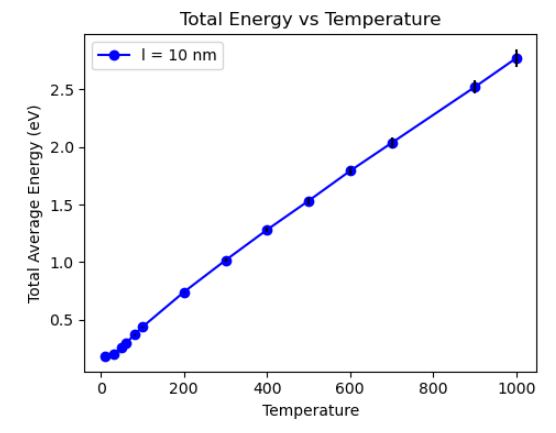
\includegraphics[width = 0.7 \linewidth]{EANDT.png}
    \caption{Curve of the average Energy of the system at equilibrium respect to the temperature of the thermal bath with its error bars, this curve is the result of the average energy of 32 different runs of the simulation in a parallel implementation.}
    \label{fig:epar}
\end{figure}

 The code distributes a specified number of simulation runs among processes, each handling simulations for assigned temperatures independently. Results are stored locally on each process and later gathered by the root process to create a (.csv) file. Subsequently, this file is copied to the local folder for analysis by another program. Utilizing MPI's distributed computing approach, the program optimizes the performance. 



\begin{figure}[h!]
    \centering
    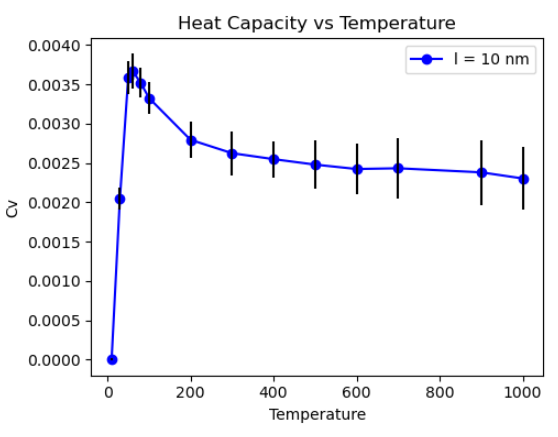
\includegraphics[width = 0.7 \linewidth]{CVANDTEMP.png}
    \caption{Curve of the average heat capacity of the system at equilibrium respect to the temperature of the thermal bath with its error bars, this curve is the result of the average heat capacity of 32 different runs of the simulation in a parallel implementation.}
    \label{fig:cvpar}
\end{figure}


The simulation was executed on a cluster featuring 8 CPUs. Each processor managed 4 simulation runs, totaling 32 runs. This parallel computing strategy notably reduced the computing time to 274.7 seconds, less than one-sixth of the time required in a serial computing scenario to obtain the same volume of data. 

Remarkably, the results obtained from parallel computation closely matched those from serial computation, accompanied by error bars too. The linear progression of total energy with increasing temperature follows theoretical expectations, reflecting the system's sensitivity to temperature variations (Fig. \ref{fig:epar}). Additionally, the smooth curve observed in the heat capacity graph (Fig. \ref{fig:cvpar}), presents an averaged fit that captures the response of system particles to energy transitions between levels. This representation offers deeper insight into the system's dynamic behavior under varying temperature conditions and confirming the accuracy and reliability of the parallel simulation adapted from the initial solution. 

\subsection{Error Analysis}
    In the analysis of results, error analysis plays a crucial role. Each data point on the graphs is accompanied by an associated error bar, representing the standard deviation calculated from the resulting values obtained on each processor for the multiple simulations. In the Figure \ref{fig:errorcv}, the error exhibits a notable increasing trend with rising temperature. This is primarily attributed to the stochastic nature of the calculated values, resulting in higher uncertainty on the heat capacity, particularly at elevated temperatures.
    \begin{figure}[!h]
        \centering
        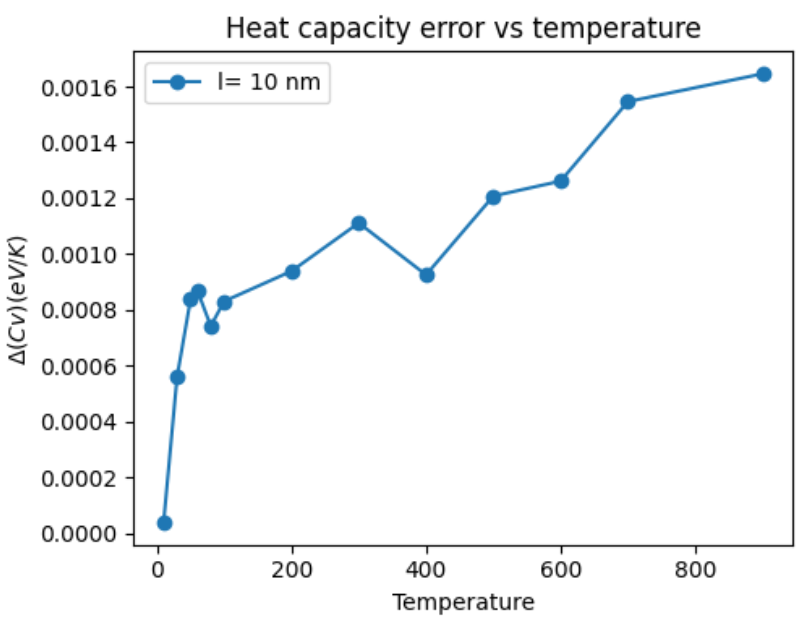
\includegraphics[width=0.7\linewidth]{ERRORCVFV.png}
        \caption{Behaviour of the heat capacity error as the temperature increase.}
        \label{fig:errorcv}
    \end{figure}
    
    Regarding the energy error respect to temperature, Figure \ref{fig:errorenergy}, shows a linear increase in error with temperature. However, the error propagation remains relatively low compared to the heat capacity uncertainty for high temperatures. This suggests that the total energy measurements yield highly reliable results, with the averaging over numerous calculations enabling accurate predictions of the system's behavior
            
    \begin{figure}[!h]
         \centering
         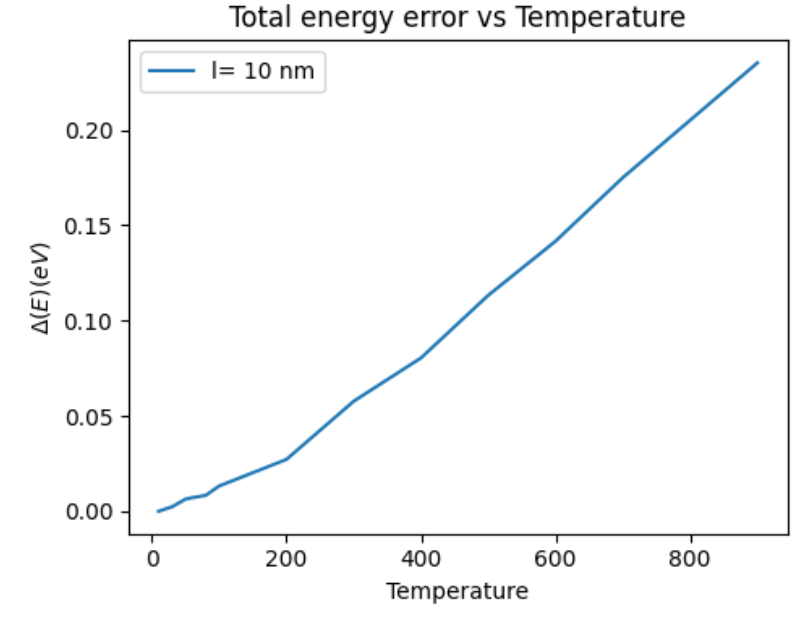
\includegraphics[width=0.7\linewidth]{ERRORENERGY.png}
        \caption{Behaviour of the energy error as the temperature increase.}
        \label{fig:errorenergy}
    \end{figure}
\subsection{Computing Times:}
The magic command \%\%time in Jupyter notebooks is a convenient way to measure the execution time of code block. According to this, the processing times for both approaches evaluated here, serial and paralell, are presented in Table \ref{tab:my-table}.

\begin{table}[!h]
\centering
\resizebox{\columnwidth}{!}{%
\begin{tabular}{|l|l|l|l|l|l|l|}
\hline
\textbf{Type}   & \textbf{n} & \textbf{Runs} & \textbf{Total Time(s)} & Wall Time & User Time & System Time \\ \hline
\textit{Serial} & 1          & 32            & 220.8s                 & 3min 40s  & 3min 33s  & 495 ms      \\ \hline
\textit{MPI}    & 8          & 4             & 274.7                  &           &           &             \\ \hline
\end{tabular}%
}
\caption{}
\label{tab:my-table}
\end{table}

\begin{itemize}
    \item [*] \textit{User Time:} Total CPU time executing user instructions, including code and function calls.
    \item [*] \textit{System Time:} Total CPU time executing system-related tasks, like handling inputs/outputs or managing resources.
    \item [*] \textit{Total Time:} Sum of user and system time, indicating overall CPU time consumed.
    \item [*] \textit{Wall Time:} Actual elapsed time from start to end of script execution, including waiting for resources and libraries. 
    
\end{itemize}

\subsection{Scalability}
   It refers to a system's ability to handle increasing workloads of datasets efficiently. In serial computing, scalability can be limited by factors such as processing power, memory constraints, and execution time. When simulations or parameter spaces expand, serial implementations may struggle to meet increasing demands, leading to prolonged computation times and potential resource constraints. 
   On the other hand, parallel computing offers scalability advantages by enabling concurrent executions of computations, which reduces the time required to handle larger simulations or parameter spaces, such as those encountered in thermal well simulations or similar scenarios. Additionally, as the number of processors or nodes in the cluster scales up, this code can be adapted to accommodate larger simulations or parameter spaces, ensuring efficient utilization of computational resources 
   \cite{robey_parallel_nodate}   \cite{prasad_scalability_2018}.

\section{CONCLUSIONS}
\begin{itemize}
    \item The initial implementation of the Monte Carlo code demonstrates significant potential as a tool for simulating complex phenomena in statistical physics.

    \item Modern computing routines and facilities have limitations. Serial architecture fails to provide efficient computing times and resource savings despite continuous algorithm performance improvements. Parallel computing allows simulations to process and generate large amounts of data quickly.
    \item This capability supports more robust analysis and ensures statistically significant results.

    \item Parallelism enables scaling up problem sizes to dimensions previously unattainable with serial applications. Increased compute resources allow for larger problem sizes, facilitated by greater amounts of main memory, disk storage, and CPUs.

    \item Shifting multimedia applications to run on GPUs instead of the main CPU units enhances energy efficiency while improving performance

    \item The determination of heat capacity for this set of potential wells paves the way for exploring more complex systems, such as quantum dots or molecular clusters. This advancement allows for a more precise description by interconnecting the wells and accurately defining transition probabilities.

\end{itemize}

\section{REFERENCES}
\nocite{*}
%\bibliographystyle{}
\bibliography{bibliog} % Replace "references" with the name of your .bib file

\end{document}
%
